\documentclass[]{article}
\usepackage{graphicx}
\usepackage{amsmath}
%opening
\title{CSC420 Assignment 1}
\author{Alex (Kao-Tsun) Chang}


\begin{document}

\maketitle


\section{}
\textbf{(a)} $\delta(u,v) =    \left\{
\begin{array}{ll}
      1 & $when $u=0$ and  $v=0 \\
      0 & $otherwise $ \\
\end{array} 
\right.$ \\
\textbf{ (b) }  $\delta(u-m,v-n) =   \left\{
\begin{array}{ll}
      1 & $when $u=0$ and  $v=0 \\
      0 & $otherwise $ \\
\end{array} 
\right.$ \\
\\
\\
\textbf{(c)}
 \begin{figure}[h!]
 \centering
  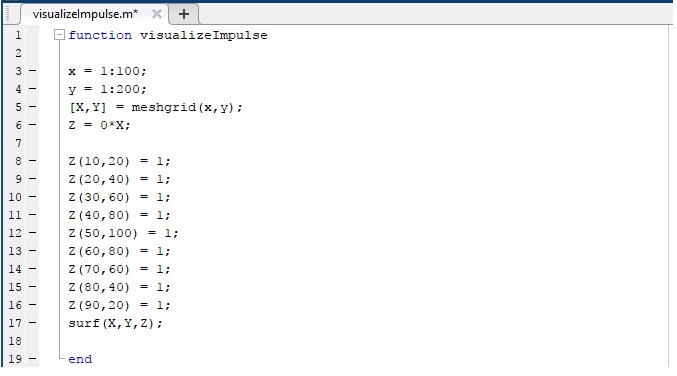
\includegraphics[width=1.15\textwidth]{img/impulsematlab.jpg}
 \caption{Matlab code}
 \end{figure}
  \begin{figure}[h!]
  \centering
   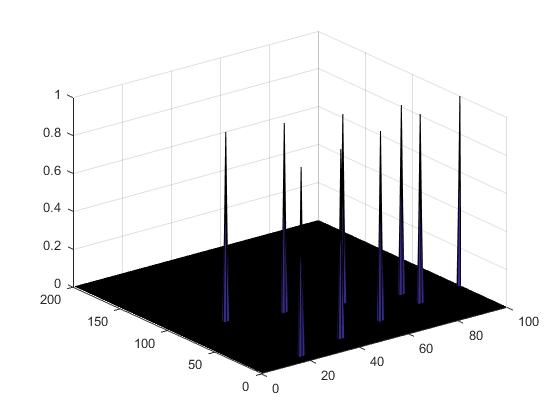
\includegraphics[width=1.15\textwidth]{img/impulse.jpg}
  \caption{Output}
  \end{figure}
\\\\\\\\\\
\textbf{(d)} $f(u,v) = \sum_{i=1}^{m} \sum_{j=1}^{n}
f(u_{i}, v_{j})\delta(u-u_{i}, v-v_{j})$
\section{}
\textbf{(a)} The computational cost of computing convolution is $O(m^{2}n^{2})$. This is because there are $n * n = n^{2}$ pixels which needs to be multiplied with $m * m = m^{2}$ pixels in the filter
\\
\\
\textbf{(b)} If h is a seperable filter into 2 $m * 1 $ sized filters, then the computational cost is $2m$ multiplied with $n * n$ pixels, which is $O(mn^{2})$
\\
\\
\textbf{(c1)} $F_{1}$ is not seperable because using the matlab function svd(F1), we can see that the output $S1$ does not only have one singular non-zero value. It must have only one singular non-zero value in the matrix as a requirement to be seperable.
 \begin{figure}[h!]
 \centering
  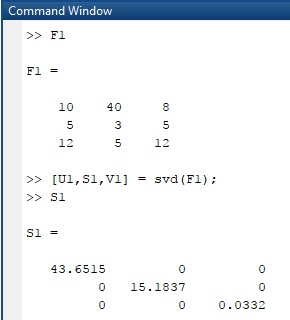
\includegraphics[width=0.85\textwidth]{img/svdF1.jpg}
 \caption{Matlab code}
 \end{figure}
\\\\\\\\\\\\
\\\\\\\\\\\\
\\\\\\\\\\\\
\\
\\
\textbf{(c2)} $F_{2}$ is seperable because it has only one singular non-zero value from the output of svd(F2)
 \begin{figure}[h!]
 \centering
  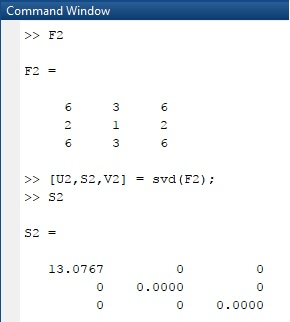
\includegraphics[width=0.85\textwidth]{img/svdF2.jpg}
 \caption{Matlab code} 
 \end{figure}
 The matrix can be written as these 2 seperable filters \\
\\
$ F_{a} =
 \begin{bmatrix}
     3, & 1, & 3 \\
 \end{bmatrix}
$ \\
$ F_{b} = 
 \begin{bmatrix}
     2, & 1, & 2 \\
 \end{bmatrix}
$
\\\\\\\\\\\\\\.
\section{}
 \begin{figure}[h!]
  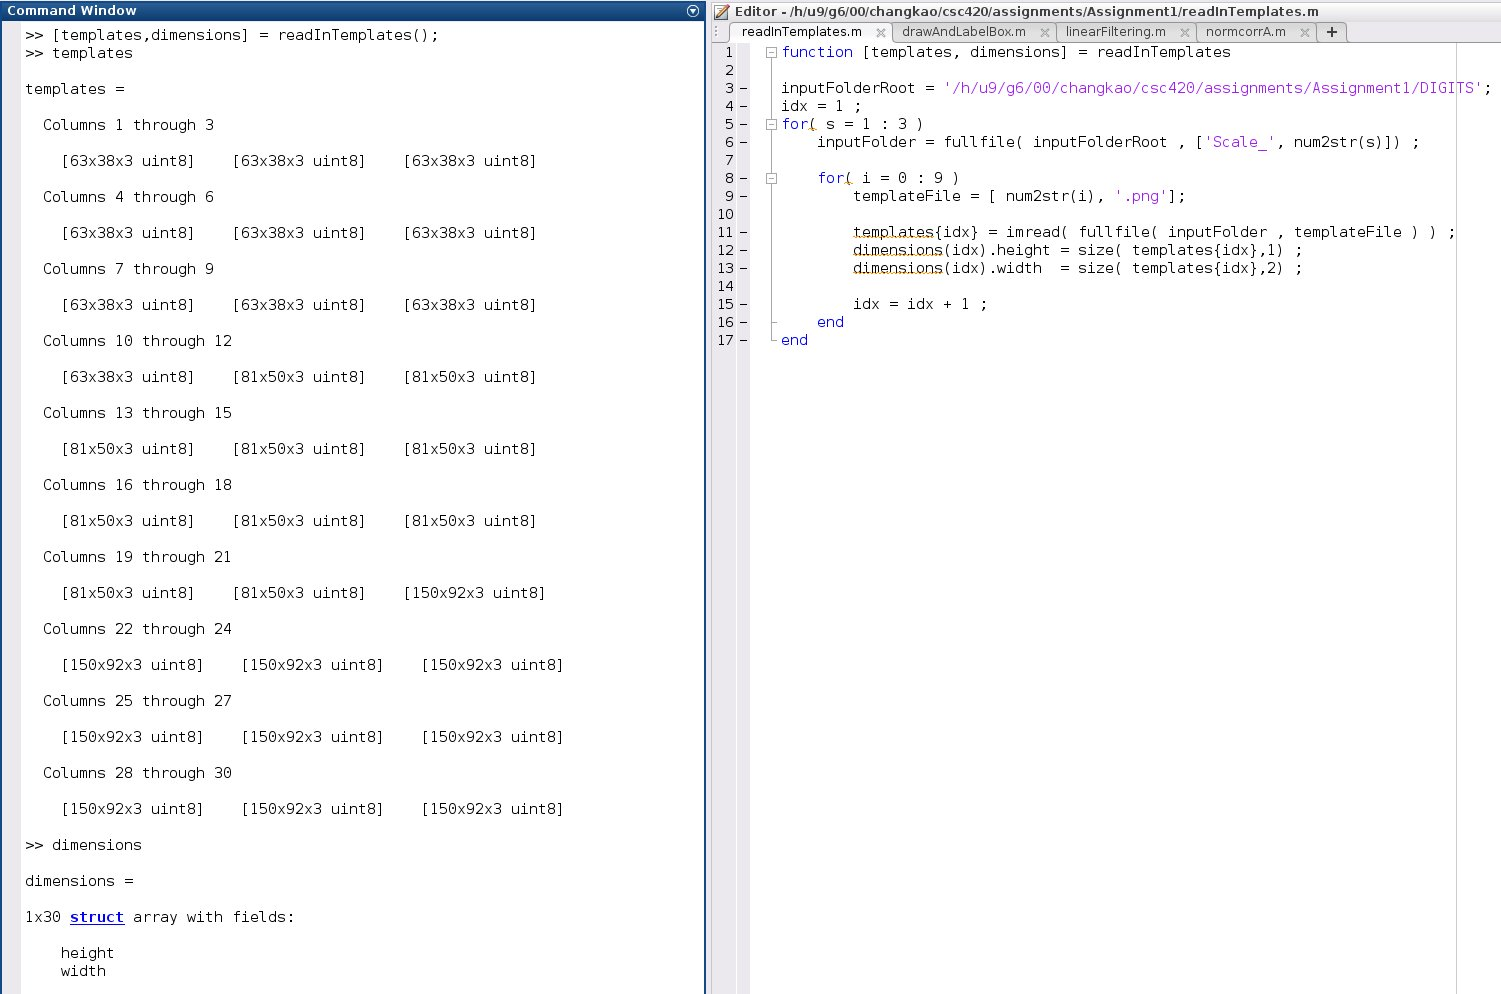
\includegraphics[width=1.32\textwidth]{img/3b.jpg}
 \caption{Code for 3b}
 \end{figure}
  \begin{figure}[h!]
   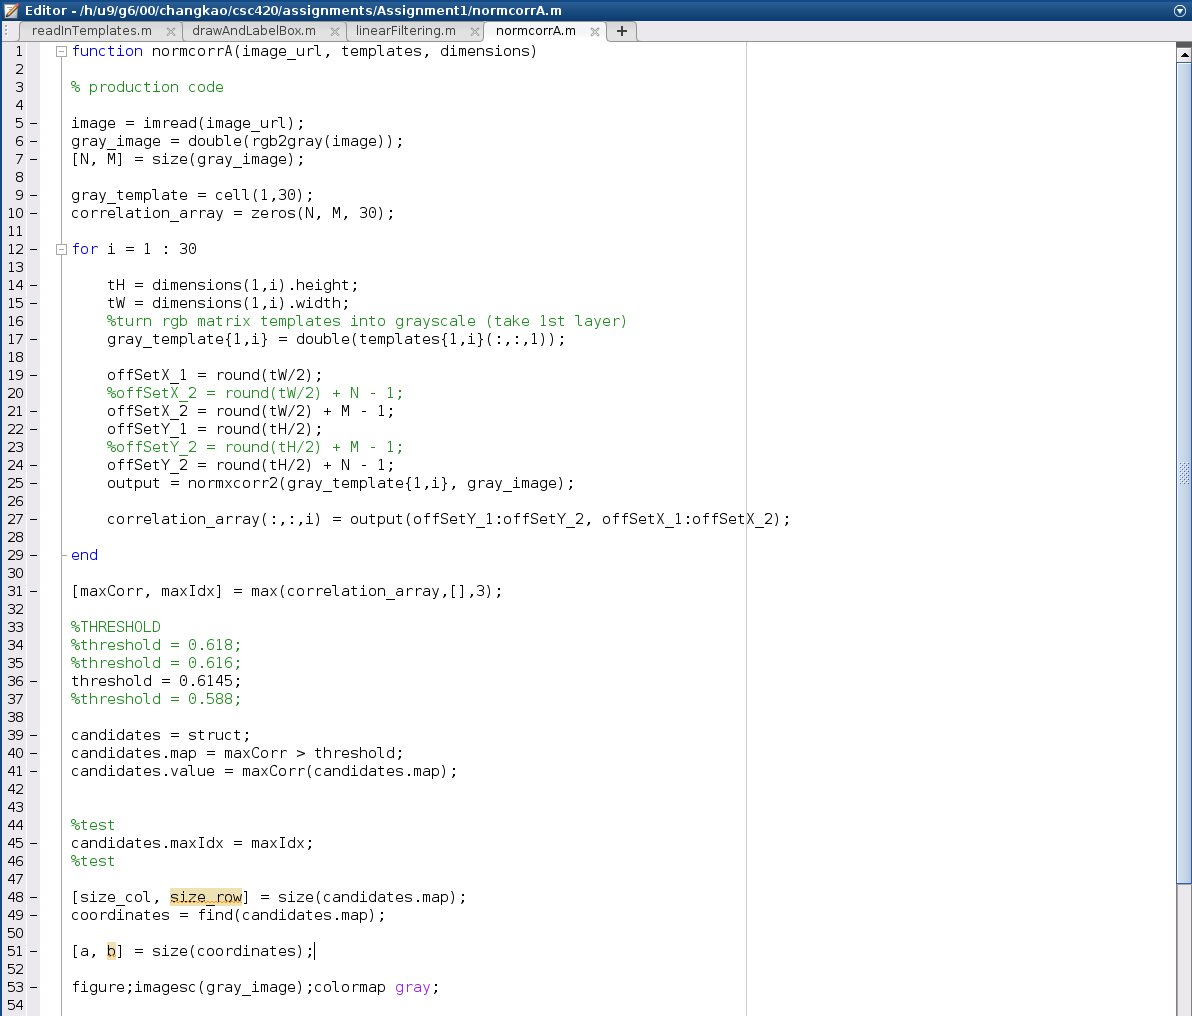
\includegraphics[width=1.32\textwidth]{img/code1.jpg}
  \caption{Matlab code part 1}
  \end{figure}
   \begin{figure}[h!]
    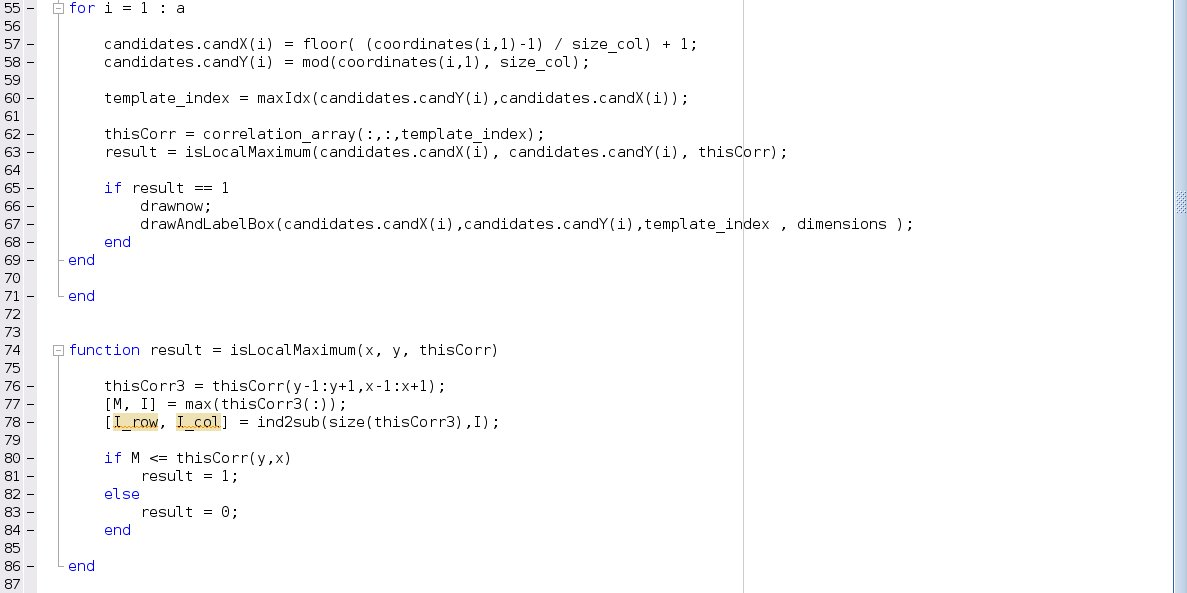
\includegraphics[width=1.32\textwidth]{img/code2.jpg}
   \caption{Matlab code part 2}
   \end{figure}
    \begin{figure}[h!]
     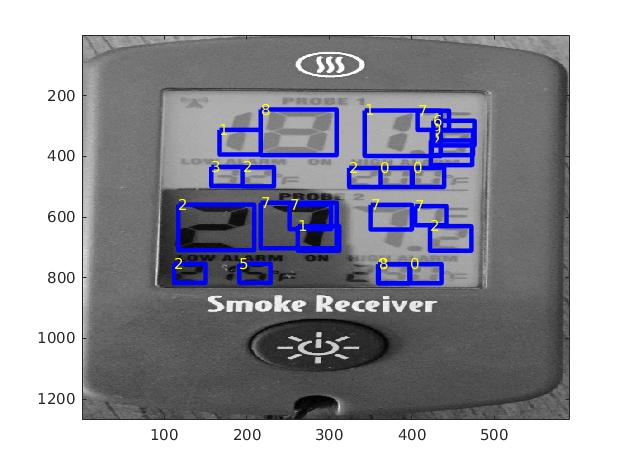
\includegraphics[width=1.32\textwidth]{img/output06145.jpg}
     \caption{Output with threshold = 0.6145}
    \pagebreak
    \textbf{(3v)}
     \\\\ The threshold used was 0.6145, the numbers correctly identified were 1,2,3,7,8
    Most of the numbers are correctly identified, only the 1 and 2 in the picture were missed and not matched \\\\
    \pagebreak
    \textbf{(3vi)}
    \\\\ If we crop our own templates from the picture, we would get better matching because the number templates would have the same intensity as the numbers on the actual image. Thus matching would become more accurate.
    \end{figure}


\end{document}
